\documentclass[xcolor=dvipsnames, aspectratio=169]{beamer}
\usepackage[T1]{fontenc}

\usepackage{amsmath, amsfonts, amsthm, amssymb, mathtools}

\usepackage{fontspec}
\usepackage[mathrm=sym, mathbf=sym]{unicode-math}
\setmainfont{FiraGO}
\setmathfont{Fira Math}
\setmathfont{Latin Modern Math}[range={\mathcal}]
\setmathfont{Fira Math}[range=]
\newfontfamily{\firaGo}{FiraGO}

\usepackage{graphicx}
\usepackage{float}
\usepackage{bookmark}
\usepackage{enumitem}
\usepackage{tabularray}

\usepackage{tikz}
\usepackage{pgfplots}
\usetikzlibrary{intersections, angles, calc, positioning}

\definecolor{softyellow}{RGB}{252, 222, 165}
\definecolor{bgg}{HTML}{fafafa}
\definecolor{bbg}{HTML}{23373b}
\definecolor{orang}{HTML}{eb811b}

\usepackage{tcolorbox}
\tcbuselibrary{skins}
\newtcolorbox{marker}[1][]{enhanced,
before skip=2mm,after skip=3mm,
boxrule=0.4pt,left=5mm,right=2mm,top=1mm,bottom=1mm,
colback=yellow!50,
colframe=yellow!20!black,
sharp corners,rounded corners=southeast,arc is angular,arc=3mm,
underlay={%
\path[fill=tcbcolback!80!black] ([yshift=3mm]interior.south east)--++(-0.4,-0.1)--++(0.1,-0.2);
\path[draw=tcbcolframe,shorten <=-0.05mm,shorten >=-0.05mm] ([yshift=3mm]interior.south east)--++(-0.4,-0.1)--++(0.1,-0.2);
\path[fill=yellow!50!black,draw=none] (interior.south west) rectangle node[white]{\huge\bfseries !} ([xshift=4mm]interior.north west);
},
drop fuzzy shadow,#1}

\usepackage{polyglossia}
\setdefaultlanguage{portuguese}
\usepackage{csquotes}
\usepackage[backend=biber, doi=false]{biblatex}
\addbibresource{bibliography.bib}

\newcommand{\bx}{\mathbf{x}}
\newcommand{\bc}{\mathbf{c}}
\newcommand{\bz}{\mathbf{0}}
\newcommand{\bb}{\mathbf{b}}

\title{Difusão com barreira}
\author{Bruno Sant'Anna\\Jacineide Aquino}
\date{4 de abril de 2024}
\institute{Universidade Federal de Sergipe}

\usetheme[progressbar=foot, block=fill]{metropolis} % https://linorg.usp.br/CTAN/macros/latex/contrib/beamer-contrib/themes/metropolis/doc/metropolistheme.pdf

\setsansfont[BoldFont={Fira Sans SemiBold}]{Fira Sans Book}
\setmonofont{Iosevka Custom Semibold}

\begin{document}
    \metroset{titleformat frame=smallcaps}
    \begin{frame}   
        \maketitle
        \begin{tikzpicture}[remember picture, overlay]
            \node (pic) at ($(current page.east) + (-2.5, 0)$) {
\includegraphics[height=0.6\paperheight]{ufs_vertical_positiva.eps}};
            \filldraw[bgg] (pic.south east) rectangle (pic.north west);
            \node at ($(current page.east) + (-2.5, 0)$) {
\includegraphics[height=0.6\paperheight]{ufs_vertical_positiva.eps}};
        \end{tikzpicture}
    \end{frame}
    \section{Introdução}
    \begin{frame}
        \frametitle{Equações elípticas e o problema de difusão}
        Uma equação diferencial parcial \textsc{edp} é uma equação que relaciona funções e suas derivadas parciais, envolvendo duas ou mais variáveis independentes.

        Um tipo de \textsc{edp} são as equações elípticas que se caracterizam pela propagação de suas propiedades físicas em todas as direções. Essas, pode ser usadas em problemas de equilibrio, difusão, pressão, entre outros. 

        Mais especificamente a equação estudada nesse trabalho foi a \textbf{equação de Poisson} dada por
        \[
            \Delta u = \dfrac{\partial^2 u}{\partial x^2} + \dfrac{\partial^2 u}{\partial y^2} = f(x,y)
        \]
        Para encontrar a solução aproximada da equação diferencial, utilizamos o metodo das diferenças finitas.
    \end{frame}
    \begin{frame}
        \frametitle{Método Numérico}
        \begin{columns}
            \begin{column}{0.6\textwidth}
                Considere a equação $\Delta u = f(x,y)$ em um domínio $\Omega = [a,b] \times [c,d]$, podemos discretizar esse domínio, escolhendo passos $h$ e $k$ para o eixo $x$ e $y$ respectivamente, de forma que os intervalos possam ser divididos em $N$ e $M$ partes iguais, essa discretização será representada por uma malha de pontos no plano $xy$. Os pontos na borda são dados pela condição de fronteira, enquanto os pontos interiores serão aproximados pelo método numérico.    
            \end{column}
            \begin{column}{0.4\textwidth}
                \begin{tikzpicture}
                    \draw[thick] (0,0) grid[step=0.5] (3,4);
                    \draw[thick, -stealth] (-0.5,-0.75) -- (-0.5,4.5);
                    \draw[thick, -stealth] (-0.75,-0.5) -- (3.5,-0.5);
                    \node (y0d) at (-0.5,-0.02) {--};
                    \node at (y0d.west) {$y_0$};
                    \node (ydd) at (-0.5,3.98) {--};
                    \node at (ydd.west) {$y_M$};
                    \node (x0d) at (0,-0.5) {|};
                    \node at ($(x0d.south) + (0,-0.05)$) {$x_0$};
                    \node (xdd) at (3,-0.5) {|};
                    \node at ($(xdd.south) + (0,-0.05)$) {$x_N$};
                \end{tikzpicture}
            \end{column}
        \end{columns}
    \end{frame}
    \begin{frame}
        Por meio da expansão em série de Taylor, podemos encontrar as formulas de diferenças centradas para as derivadas parciais
        \[
            \dfrac{\partial^2 u}{\partial x^2}(x_i, y_j) \approx \frac{u(x_{i+1}, y_j) - 2u(x_i, y_j) + u(x_{i-1}, y_j)}{h^2} 
        \]
        \[
            \dfrac{\partial^2 u}{\partial y^2}(x_i, y_j) \approx \frac{u(x_i, y_{j+1}) - 2u(x_i, y_j) + u(x_i, y_{j-1})}{k^2}
        \]
    \end{frame}
    \begin{frame}
        Por simplicidade, escrevemos $u(x_i,y_j) = u_{ij}$
        \[
            \frac{u_{i +1 \, j} - 2u_{ij} + u_{i-1\,j}}{h^2} + \frac{u_{i \, j+1} - 2u_{ij} + u_{i \, j-1}}{k^2} = f(x_i, y_j)
        \]
        Organizando os termos ficamos com a equação
        \[
            2\left( \lambda + 1 \right) u_{ij} - u_{i-1 \, j} - u_{i+1 \, j} - \lambda \left( u_{i \, j-1} + u_{i \, j+1} \right) = -h^2 f(x_i, y_j)
        \]
        onde $\lambda = \left( \frac{k}{h} \right)^2$, para cada $i = 1, 2, \dots, N-1$ e $j = 1, 2, \dots, M-1$.
    \end{frame}
    \begin{frame}
        \begin{columns}
            \begin{column}{0.6\textwidth}
                Utilizamos pontos ao redor de $w_{ij}$ para encontrar uma solução aproximada. Nesse caso será necessário resolver um sistema de equações lineares para calcular todos $w_{ij}$ no interior da malha.
            \end{column}
            \begin{column}{0.4\textwidth}
                \begin{tikzpicture}
                    \draw[thick] (0,0) grid[step=1] (3,4);
                    \draw[thick, teal] (0,0) -- (3,0);
                    \draw[thick, purple!50!black] (0,0) -- (0,4);
                    \draw[thick, green!50!black] (3,0) -- (3,4);
                    \draw[thick, blue!50] (3,4) -- (0,4);
                    \draw[thick, -stealth] (-0.5,-0.75) -- (-0.5,4.5);
                    \draw[thick, -stealth] (-0.75,-0.5) -- (3.5,-0.5);
                    \filldraw[orange] (1,1) circle (0.1) node[above right] {$w_{ij}$};
                    \filldraw (1,2) circle (0.08) node[above right] {$w_{i\,j+1}$};
                    \filldraw (1,0) circle (0.08) node[above right] {$w_{i\,j-1}$};
                    \filldraw (0,1) circle (0.08) node[above right] {$w_{i-1\,j}$};
                    \filldraw (2,1) circle (0.08) node[above right] {$w_{i+1\,j}$};
                \end{tikzpicture}
            \end{column}
        \end{columns}
    \end{frame}
    \section{Resultados}
    \begin{frame}
        \frametitle{Caso sem barreira}

        No primeiro caso utilizamos o metodo numérico de diferenças finitas para resolver a \textsc{edp} de difusão
        \[
            \left\{ 
                \begin{array}{ll}
                    -\alpha \Delta u = \sin (\pi x) \sin (\pi y) & (x,y) \in \Omega\\
                    u(x,y) = 0 & (x,y) \in \partial \Omega
                \end{array}
            \right.
        \]
        onde $\Omega = [0,1] \times [0,1]$
    \end{frame}
    \begin{frame}
        \begin{columns}
            \begin{column}{0.4\textwidth}
                Discretizando o dominio com $h = k = \frac{1}{20}$ e utilizando o algoritmo obtemos o seguinte resultado
            \end{column}
            \begin{column}{0.6\textwidth}
                \begin{center}
                    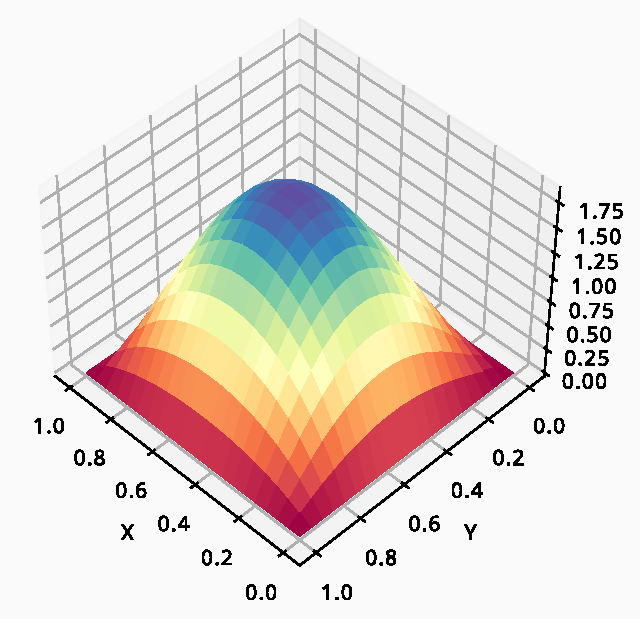
\includegraphics[width=\columnwidth]{../../difusão.pdf}
                \end{center}
            \end{column}
        \end{columns}
    \end{frame}
    \begin{frame}
        \frametitle{Caso com barreira}
        \begin{columns}
            \begin{column}{0.6\textwidth}
                Agora, introduzimos uma barreira dada pela função $g : \Omega \to \mathbf{R}$, onde $g(x,y) = 1$ quando $(x,y) \in \mathcal R = \left[ \frac{1}{3}, \frac{2}{3} \right] \times \left[ \frac{1}{3}, \frac{2}{3} \right]$.

                \medskip

                Nesse caso se $(x,y) \in \mathcal R$, temos que a solução será limitada por $g(x,y)$
            \end{column}
            \begin{column}{0.4\textwidth}
                \begin{center}
                    \begin{tikzpicture}
                        \draw[-stealth, thick] (-0.25,0) -- (3.25,0);
                        \draw[-stealth, thick] (0,-0.25) -- (0,3.25);

                        \draw[thick, fill=bbg!50] (1,1) rectangle (2,2);
                    \end{tikzpicture}
                \end{center}
            \end{column}
        \end{columns}
    \end{frame}
    \begin{frame}
        \begin{columns}
            \begin{column}{0.4\textwidth}
                Nesse caso, para melhor vizualização discretizamos o domínio com uma malha mais fina, dessa vez, $h = k = \frac{1}{30}$
            \end{column}
            \begin{column}{0.6\textwidth}
                \begin{center}
                    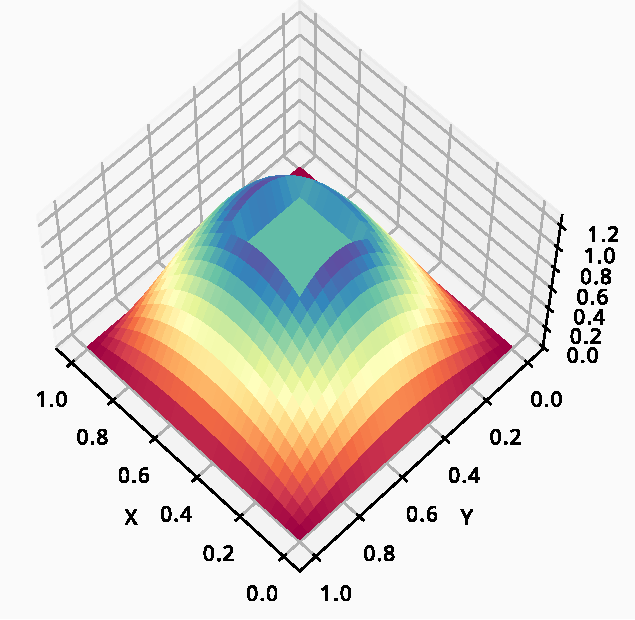
\includegraphics[width=\columnwidth]{../../difusão_barreira.pdf}
                \end{center}
            \end{column}
        \end{columns}
    \end{frame}
    \begin{frame}
        \frametitle{Algoritmo}
        \begin{center}
            \href{https://colab.research.google.com/drive/1Y1kNWiiygloHG2eUsq1QT8r1A1eB4Pjj?usp=sharing}{
\includegraphics[width=1cm]{python-svgrepo-com.pdf}}
        \end{center}
    \end{frame}
    \begin{frame}
        \nocite{*}
        \printbibliography
    \end{frame}
\end{document}